%%
%% This is file `tikzposter-template.tex',
%% generated with the docstrip utility.
%%
%% The original source files were:
%%
%% tikzposter.dtx  (with options: `tikzposter-template.tex')
%%
%% This is a generated file.
%%
%% Copyright (C) 2014 by Pascal Richter, Elena Botoeva, Richard Barnard, and Dirk Surmann
%%
%% This file may be distributed and/or modified under the
%% conditions of the LaTeX Project Public License, either
%% version 2.0 of this license or (at your option) any later
%% version. The latest version of this license is in:
%%
%% http://www.latex-project.org/lppl.txt
%%
%% and version 2.0 or later is part of all distributions of
%% LaTeX version 2013/12/01 or later.
%%


\documentclass{tikzposter} %Options for format can be included here

\usepackage{todonotes}

\usepackage[tikz]{bclogo}
\usepackage{lipsum}
\usepackage{amsmath}

\usepackage{booktabs}
\usepackage{longtable}
\usepackage[absolute]{textpos}
\usepackage[it]{subfigure}
\usepackage{graphicx}
\usepackage{cmbright}
%\usepackage[default]{cantarell}
%\usepackage{avant}
%\usepackage[math]{iwona}
\usepackage[math]{kurier}
\usepackage[T1]{fontenc}


%% add your packages here
\usepackage{hyperref}
% for random text
\usepackage{lipsum}
\usepackage[english]{babel}
\usepackage[pangram]{blindtext}

\colorlet{backgroundcolor}{blue!10}

 % Title, Author, Institute
\title{Bike Sharing Demand Prediction}
\author{Dong Zhu}
\institute{Deakin University, Australia
}
%\titlegraphic{logos/tulip-logo.eps}

%Choose Layout
\usetheme{Wave}

%\definebackgroundstyle{samplebackgroundstyle}{
%\draw[inner sep=0pt, line width=0pt, color=red, fill=backgroundcolor!30!black]
%(bottomleft) rectangle (topright);
%}
%
%\colorlet{backgroundcolor}{blue!10}

\begin{document}


\colorlet{blocktitlebgcolor}{blue!23}

 % Title block with title, author, logo, etc.
\maketitle

\begin{columns}
 % FIRST column
\column{0.5}% Width set relative to text width

%%%%%%%%%% -------------------------------------------------------------------- %%%%%%%%%%
 %\block{Main Objectives}{
%  	      	\begin{enumerate}
%  	      	\item Formalise research problem by extending \emph{outlying aspects mining}
%  	      	\item Proposed \emph{GOAM} algorithm is to solve research problem
%  	      	\item Utilise pruning strategies to reduce time complexity
%  	      	\end{enumerate}
%%  	      \end{minipage}
%}
%%%%%%%%%% -------------------------------------------------------------------- %%%%%%%%%%


%%%%%%%%%% -------------------------------------------------------------------- %%%%%%%%%%
\block{Introduction}{
  Bike sharing systems are a means of renting bicycles where the process
   of obtaining membership, rental, and bike return is automated via 
   a network of kiosk locations throughout a city. Using these systems, 
   people are able rent a bike from a one location and return it to a 
   different place on an as-needed basis. Currently, there are over 500 bike-sharing programs around the world.

  The data generated by these systems makes them attractive for researchers 
  because the duration of travel, departure location, arrival location, 
  and time elapsed is explicitly recorded. Bike sharing systems therefore 
  function as a sensor network, which can be used for studying mobility in a city. 
  In this competition, participants are asked to combine historical usage patterns 
  with weather data in order to forecast bike rental demand in the Capital Bikeshare 
  program in Washington, D.C.
    
}
%%%%%%%%%% -------------------------------------------------------------------- %%%%%%%%%%


%%%%%%%%%% -------------------------------------------------------------------- %%%%%%%%%%
\block{Dataset Description}{
\begin{itemize}
    \item
    %\emph{Group Outlying Aspects Mining}
    The competition provides hourly rental data spanning two years. For this competition, the training set is comprised of the first 19 days of each month, while the test set is the 20th to the end of the month. You must predict the total count of bikes rented during each hour covered by the test set, using only information available prior to the rental period.

    \item
    Data Fields
    \end{itemize} 
      
    \bigskip 
      \begin{tabular}{ l | l }
        \toprule
        Attribute     &  Description          \\
        \midrule
        datetime       &  hourly date + timestamp  \\
        season      & 1 = spring, 2 = summer, 3 = fall, 4 = winter\\ 
        holiday  & whether the day is considered a holiday\\
        workingday & whether the day is neither a weekend nor holiday\\
        weather    & 1: Clear,2: Mist, 3: Light Snow, Light Rain , 4: Extreme weather\\ 
        temp  & temperature in Celsius\\
        atemp  & "feels like" temperature in Celsius\\
        humidity  & relative humidity\\
        windspeed  &  wind speed\\
        casual  & number of non-registered user rentals initiated\\
        registered  & number of registered user rentals initiated\\
        count  & number of total rentals \\
    
        \bottomrule
      \end{tabular}



}
%%%%%%%%%% -------------------------------------------------------------------- %%%%%%%%%%


%%%%%%%%%% -------------------------------------------------------------------- %%%%%%%%%%

%\note{Note with default behavior}

%\note[targetoffsetx=12cm, targetoffsety=-1cm, angle=20, rotate=25]
%{Note \\ offset and rotated}

 % First column - second block


%%%%%%%%%% -------------------------------------------------------------------- %%%%%%%%%%
\block{Data Visualization}
{
\begin{itemize}
\item
Time characteristic analysis
\end{itemize} 
\vspace{-1cm} 
\begin{tikzfigure}
\centering
\selectcolormodel{rgb}
%  \missingfigure{Testing a long text string.}
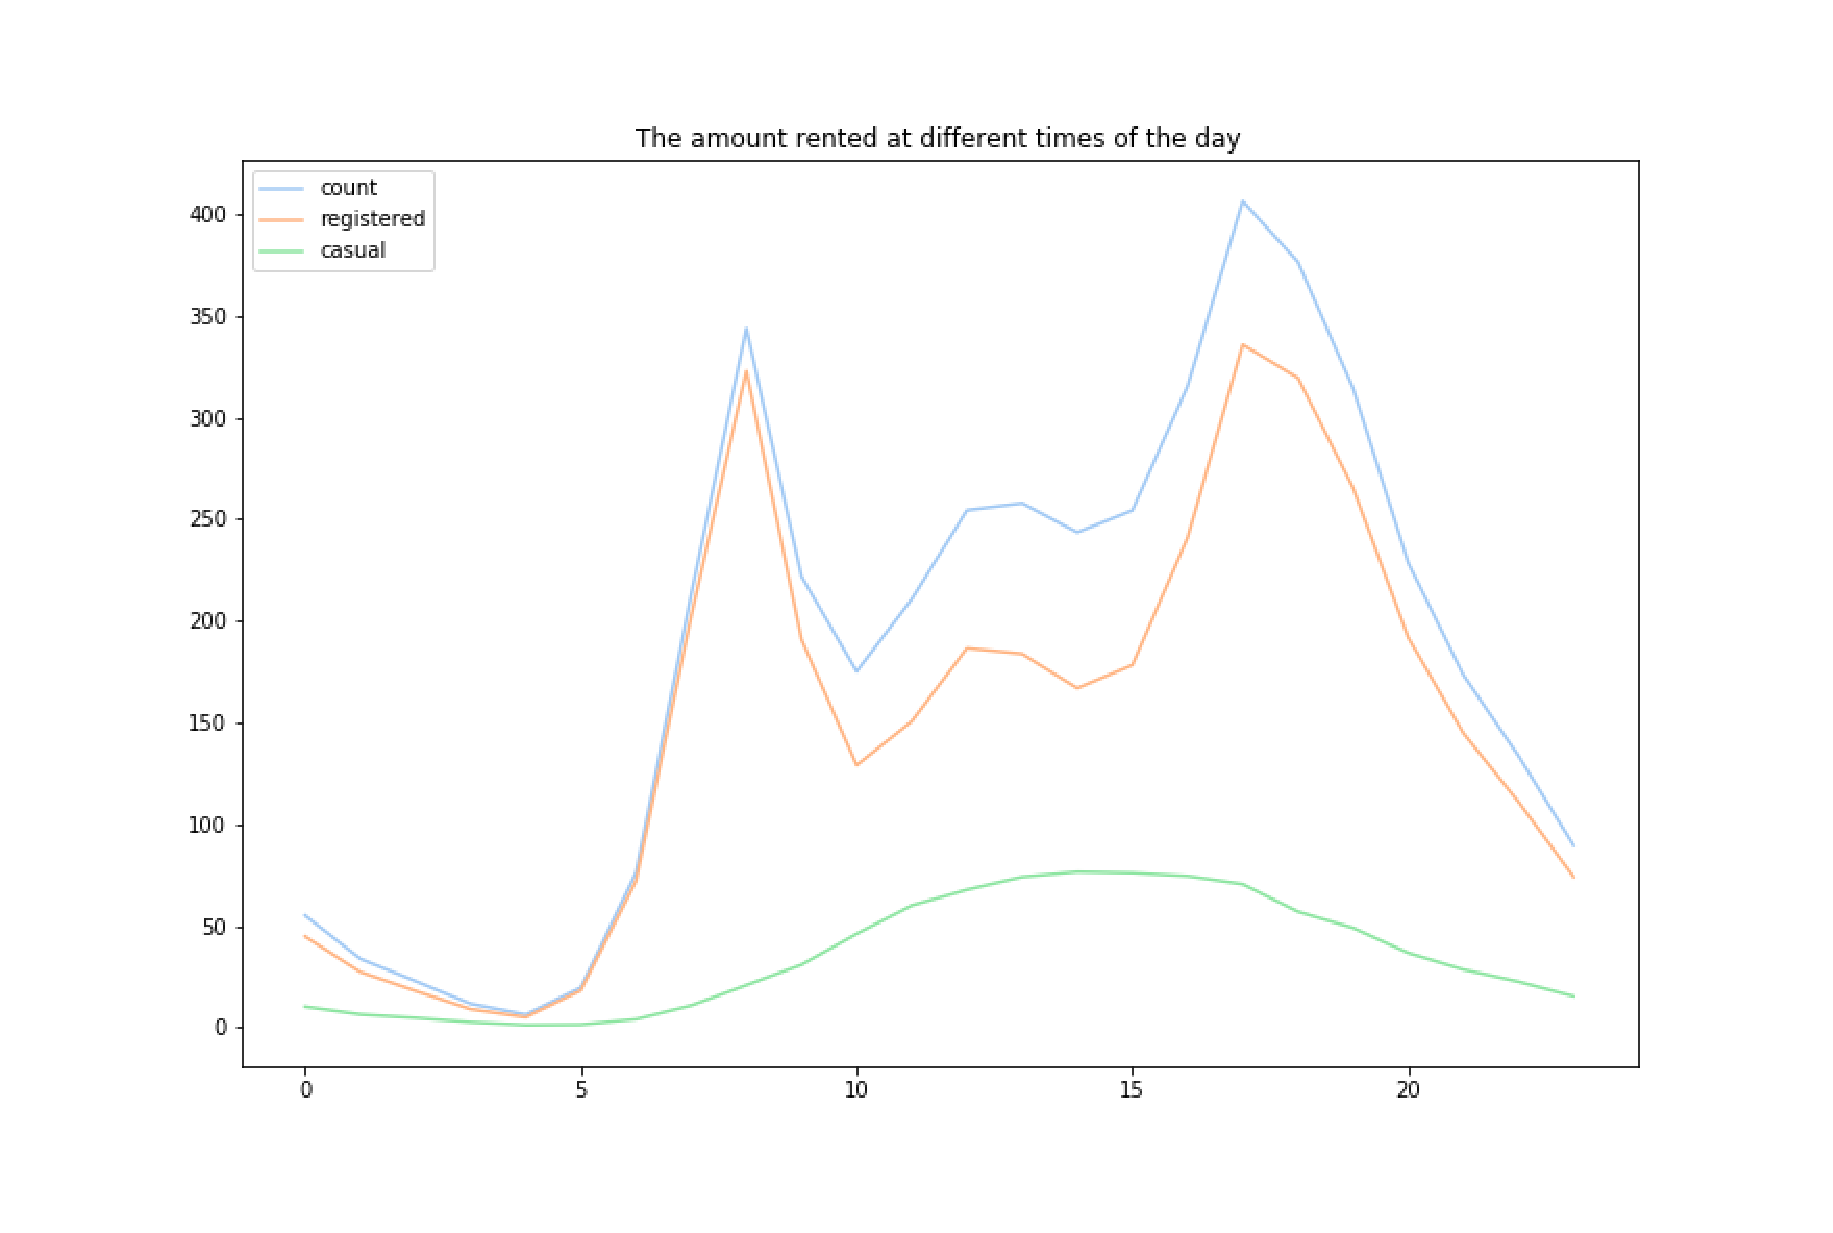
\includegraphics[width=0.2\textwidth]{figures//Time_trends_day.eps}\\
%  \caption{The amount rented at different times of the day} \label{framework}
\end{tikzfigure}
        

}
%%%%%%%%%% -------------------------------------------------------------------- %%%%%%%%%%


% SECOND column
\column{0.5}
 %Second column with first block's top edge aligned with with previous column's top.
%%%%%%%%%% -------------------------------------------------------------------- %%%%%%%%%%
\block{Data Visualization}
{

\begin{itemize}
\item
Weather characteristics analysis
\end{itemize}
\vspace{-0.8cm}
\begin{tikzfigure}
\centering
\selectcolormodel{rgb}
%  \missingfigure{Testing a long text string.}
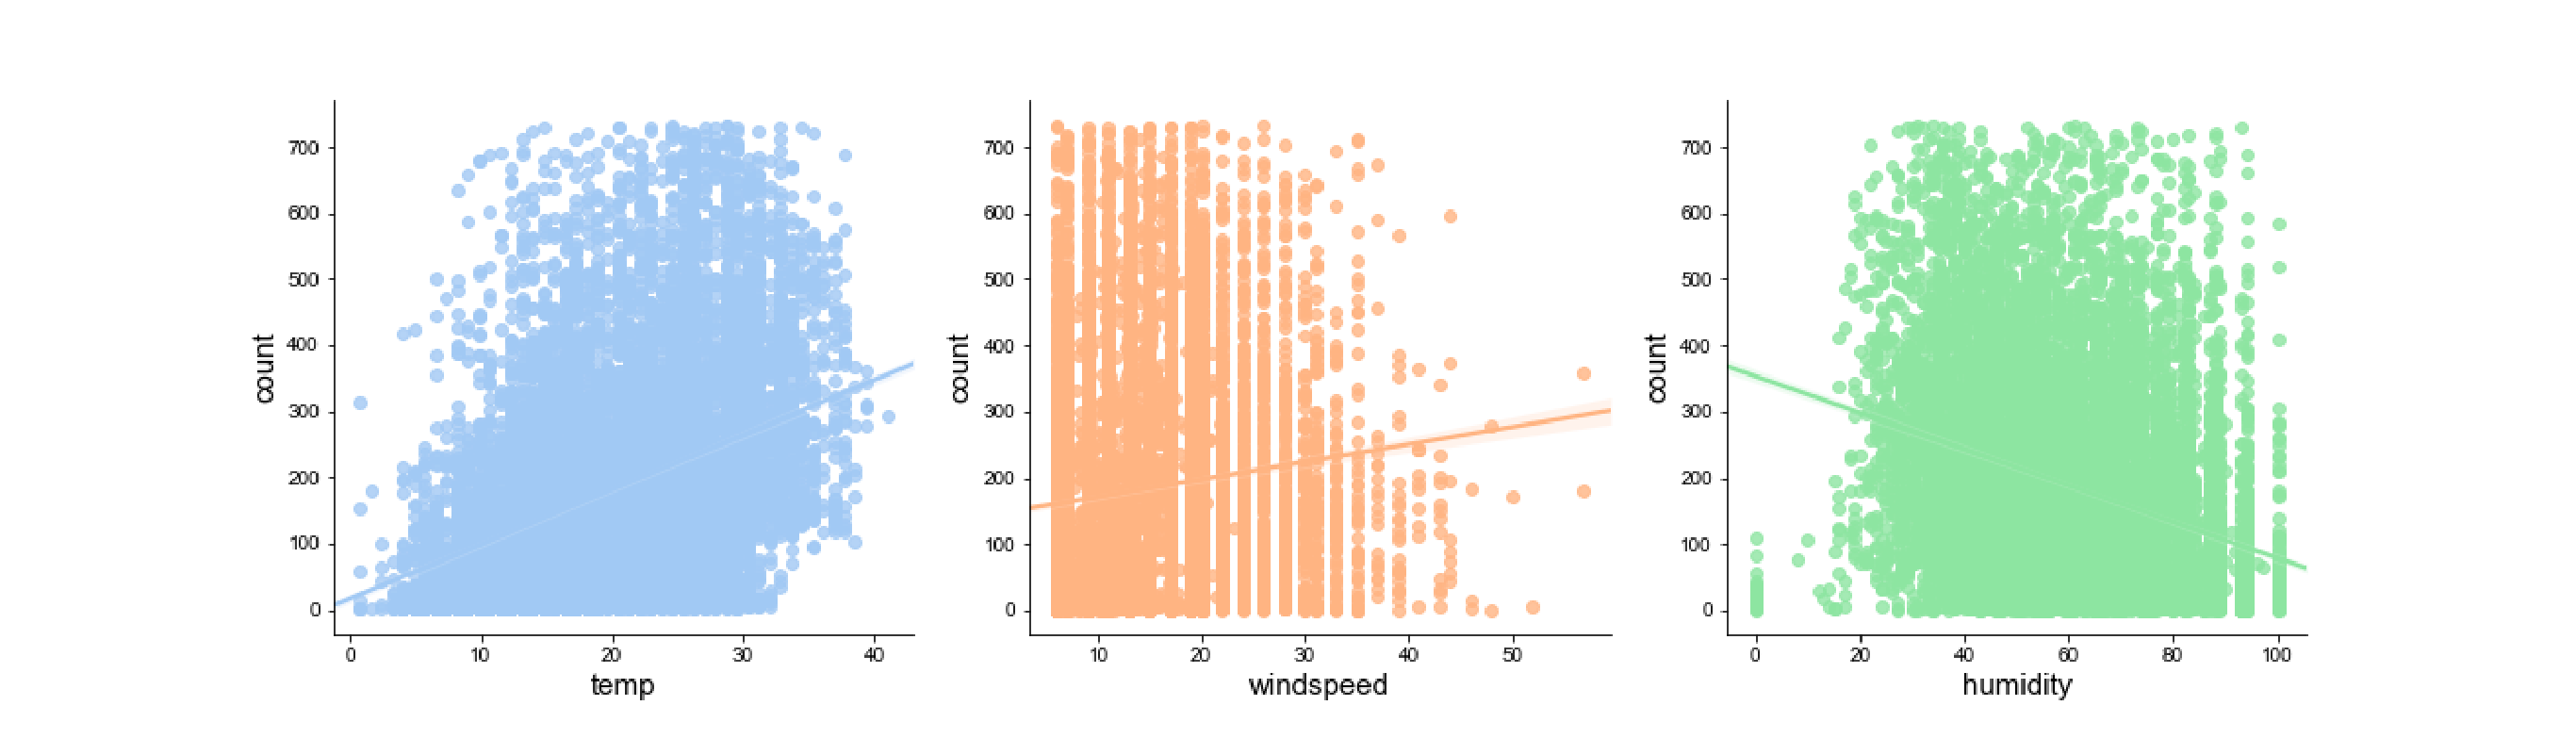
\includegraphics[width=0.4\textwidth]{figures//weather.eps}\\
%\caption{The effect of weather on rental amount} \label{framework}
\end{tikzfigure}
}
%%%%%%%%%% -------------------------------------------------------------------- %%%%%%%%%%
%%%%%%%%%% -------------------------------------------------------------------- %%%%%%%%%%
\block{Feature Selection and Feature Importance}{
\begin{description}
\item
The influence of characteristics on count is as follows:\\ 
hour>temp>atemp>humidity>month>season>year>weather>windspeed
>workingday>weekday>day>holiday
\end{description}
\vspace{-0.8cm}
\begin{tikzfigure}
\centering
\selectcolormodel{rgb}
%  \missingfigure{Testing a long text string.}
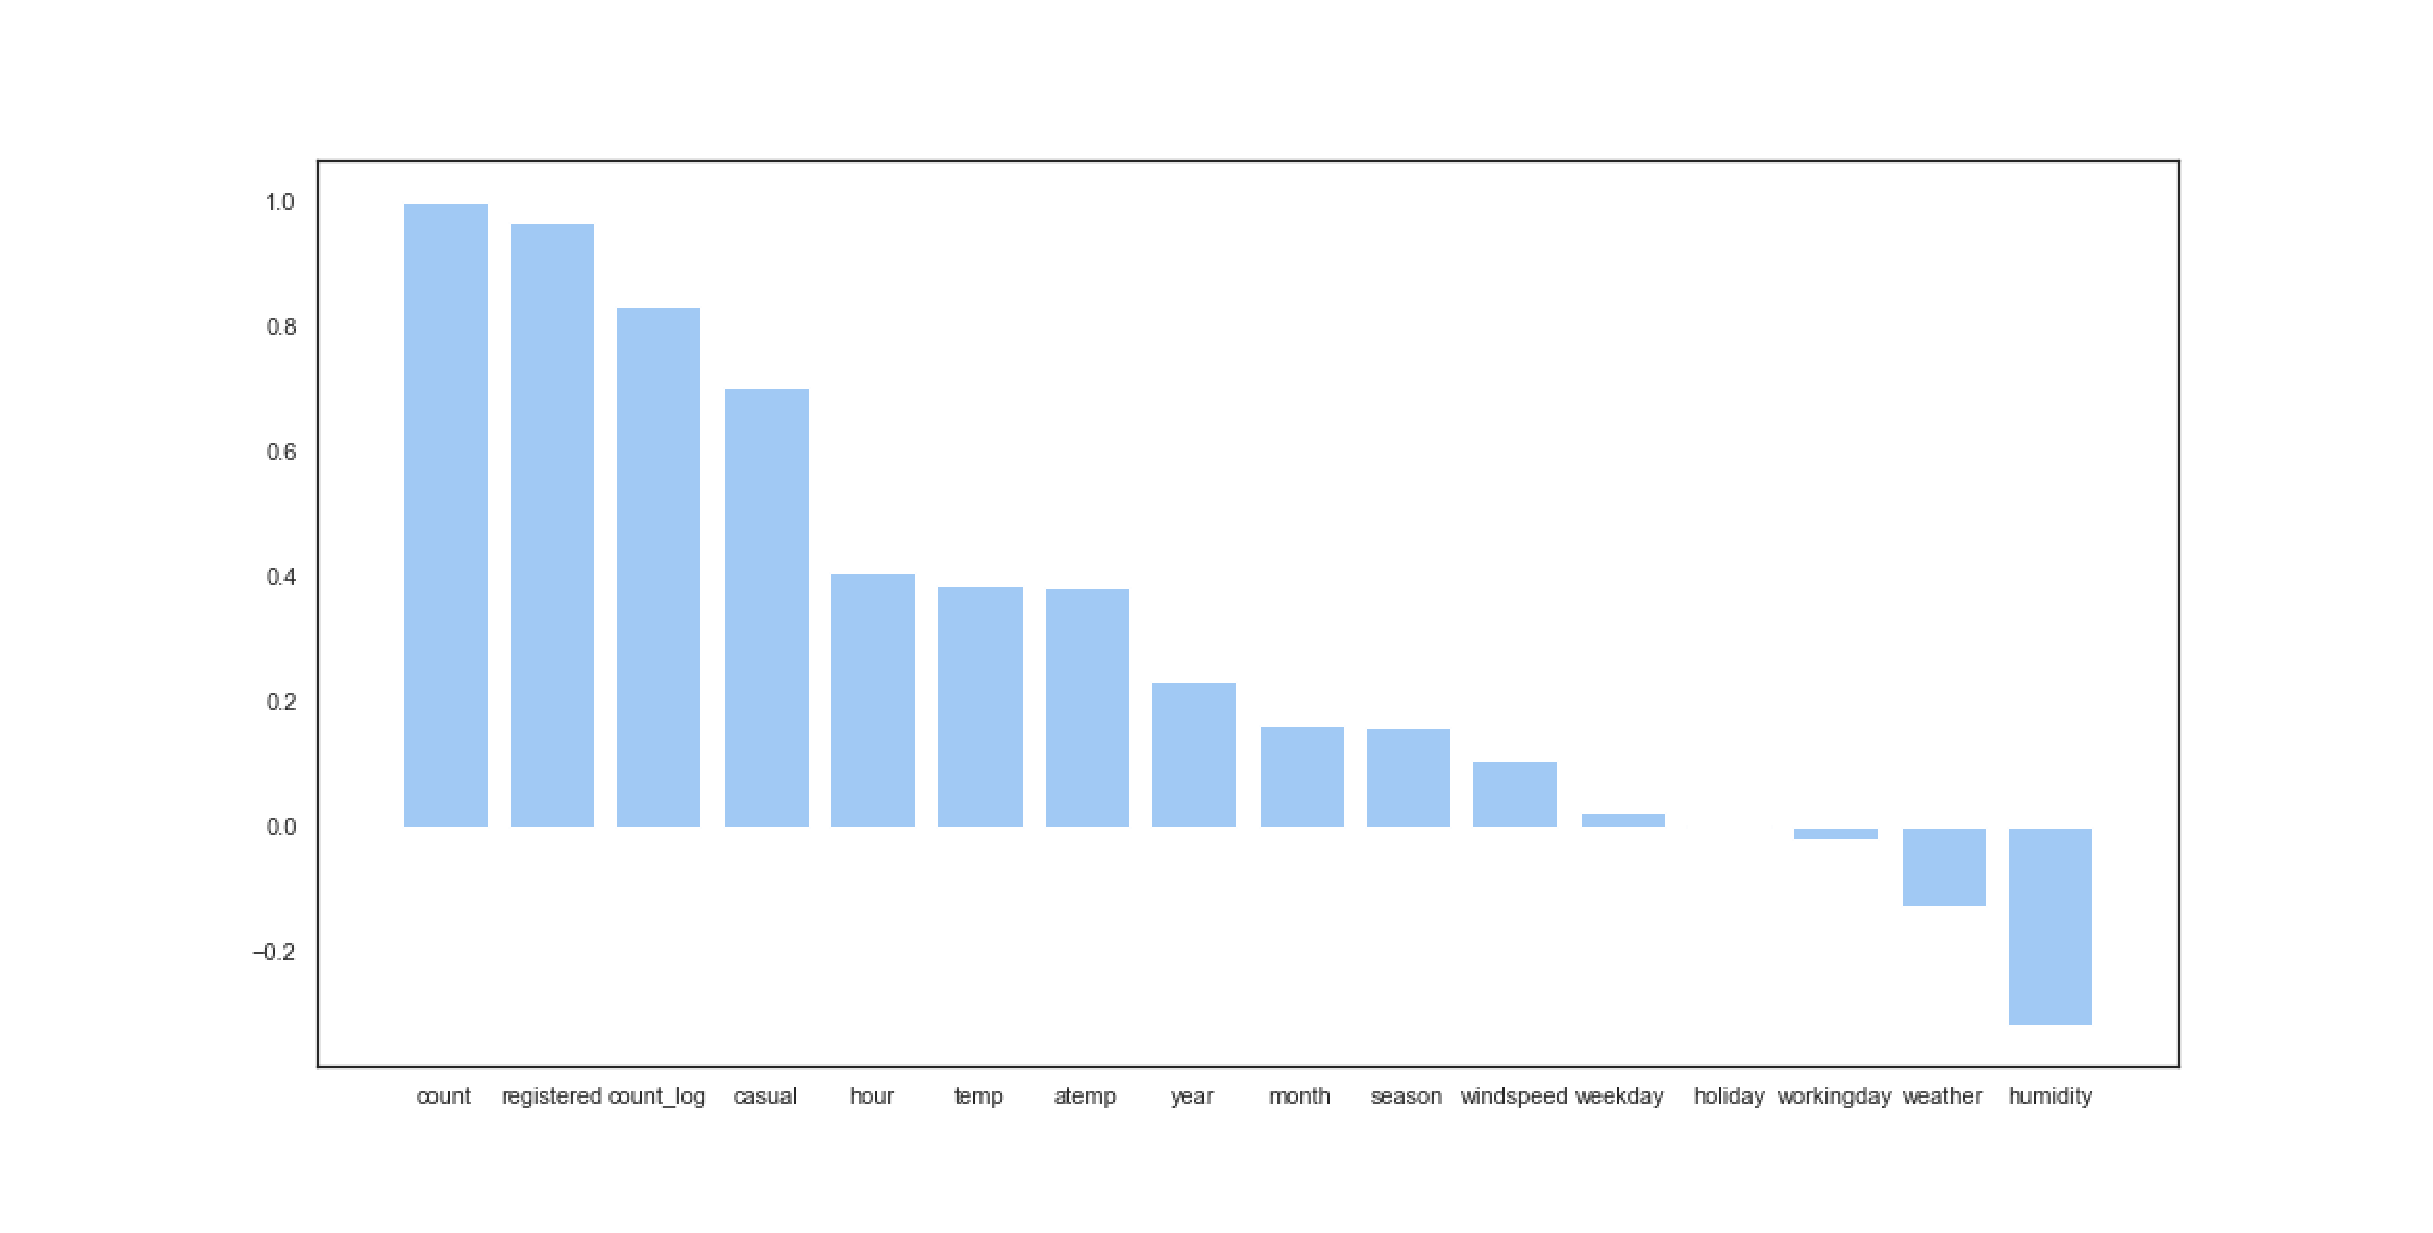
\includegraphics[width=0.4\textwidth]{figures//cor_rank.eps}\\
%\caption{Correlation rank} \label{framework}
\end{tikzfigure}

}
%%%%%%%%%% -------------------------------------------------------------------- %%%%%%%%%%
% Second column - first block


%%%%%%%%%% -------------------------------------------------------------------- %%%%%%%%%%
\block[titleleft]{Modeling and Result}
{
\begin{description}
  	\item[Model:] RandomForestRegressor
    
\end{description}
\vspace{.5cm}
\begin{tabular}{ c | c | c  }
    \toprule
    Result     &  The initial model    & After cross validation       \\
    \midrule
    Accuracy       &  0.9338   &  0.9249       \\

    MSLE      &  0.0152   &  0.0159     \\

     
     \bottomrule
\end{tabular}

}
%%%%%%%%%% -------------------------------------------------------------------- %%%%%%%%%%


% Second column - second block
%%%%%%%%%% -------------------------------------------------------------------- %%%%%%%%%%
\block[titlewidthscale=1, bodywidthscale=1]
{Conclusion}
{
\begin{description}
\item
  Cross-validation by grid search did not decrease the RMSE of the model and did not improve the accuracy of the model.
The effect did not come up to expectations.
\item
The limitation of this study is that it does not consider whether there is overfitting of the model, and further experiments can be carried out in future studies.
\end{description}
}
%%%%%%%%%% -------------------------------------------------------------------- %%%%%%%%%%


% Bottomblock
%%%%%%%%%% -------------------------------------------------------------------- %%%%%%%%%%


%\note[targetoffsetx=8cm, targetoffsety=-10cm,rotate=0,angle=180,radius=8cm,width=.46\textwidth,innersep=.1cm]{
%Acknowledgement
%}

%\block[titlewidthscale=0.9, bodywidthscale=0.9]
%{Acknowledgement}{
%}
%%%%%%%%%% -------------------------------------------------------------------- %%%%%%%%%%

\end{columns}


%%%%%%%%%% -------------------------------------------------------------------- %%%%%%%%%%
%[titleleft, titleoffsetx=2em, titleoffsety=1em, bodyoffsetx=2em,%
%roundedcorners=10, linewidth=0mm, titlewidthscale=0.7,%
%bodywidthscale=0.9, titlecenter]

%\colorlet{noteframecolor}{blue!20}
\colorlet{notebgcolor}{blue!20}
\colorlet{notefrcolor}{blue!20}
\note[targetoffsetx=-13cm, targetoffsety=-12cm,rotate=0,angle=180,radius=8cm,width=.96\textwidth,innersep=.4cm]
{
\begin{minipage}{0.3\linewidth}
\centering
\includegraphics[width=24cm]{logos/tulip-wordmark.eps}
\end{minipage}
\begin{minipage}{0.7\linewidth}
{ \centering
 The $11^{th}$ International Conference on Knowledge Science,
  Engineering and Management (KSEM 2018),
  17-19/08/2018, Changchun, China
}
\end{minipage}
}
%%%%%%%%%% -------------------------------------------------------------------- %%%%%%%%%%


\end{document}

%\endinput
%%
%% End of file `tikzposter-template.tex'.
